%!TEX root = ../template.tex
%%%%%%%%%%%%%%%%%%%%%%%%%%%%%%%%%%%%%%%%%%%%%%%%%%%%%%%%%%%%%%%%%%%%
%% chapter2.tex
%% NOVA thesis document file
%%
%% Chapter with the template manual
%%%%%%%%%%%%%%%%%%%%%%%%%%%%%%%%%%%%%%%%%%%%%%%%%%%%%%%%%%%%%%%%%%%%

\typeout{NT FILE demmon.tex}

\chapter{DeMMON}
\label{cha:demmon} 

DeMMon (Decentralized Management and Aggregation Overlay Network) is a monitoring framework which aims to tackle the needs of decentralized resource management tools. These tools, as previously mentioned, must perform resource management decisions, such as load balancing or QOS optimizations, supported by partial and localized knowledge of the system. It is the goal of this framework, through the on-demand decentralized collection, aggregation and storage of metrics in the form of time-series, to provide this knowledge base. We now detail what we believe to be the most common requirements of such tools:

\begin{enumerate} \label{enum:demmon}

    \item \textbf{Have a partial set of nodes} from the system which are nearby (according to a certain proximity heuristic). These nodes are crucial in order to perform the aforementioned localized resource management decisions. In our framework, we chose latency as the heuristic for the proximity heuristic as not only does it does not rely on external tools, such as traceroute or a reverse IP-to-geolocation service, nor does it require pre-configuration of geolocation, making it possible for all nodes' configurations to be similar (thus making the deployment of large quantities of nodes easier). \label{enum:demmon_1}
    
    \item Ensure there are ways to \textbf{obtain the aggregate value of a metric distributed across the entire system} (e.g. the total number of nodes, service replicas, among others) without having to rely on a central component. This feature is crucial for resource management tools so they, for example, maintain a desired ratio of service replicas to nodes: by simultaneously collecting both the number of nodes in the system and the number of replicas, nodes can perform local decisions such as creating or decomissioning replicas, whenever the desired ratio of reaches a certain bound. \label{enum:demmon_2}
    
    \item Having a way to perform \textbf{decentralized collection of metrics from "nearby" nodes}. This feature is useful for decentralized resource management systems as it allows nodes to perform actions such as load-balancing or QOS improvement: by collecting the metrics relative to the usage of nearby nodes, each node may decide (e.g to perform latency, or reduce the load on a saturated service) to perform service migration or service replication. \label{enum:demmon_3}
    
    \item As it is impossible to know ahead of time what information such systems would otherwise require, it is also a requirement to \textbf{be as flexible as possible in regard to the types of metrics} that are stored. This is paramount as resource management tools may need to store information in custom formats, tailored for their own needs. \label{enum:demmon_4}
    
    \item Provide ways to efficiently \textbf{propagate information} accross nodes in the system. This is useful for resource management systems, as it allow them to disseminate information using the optimized connections established by the framework. \label{enum:demmon_5}
    
    \item Ensure ways to \textbf{receive alerts} based on the collected information without resorting to periodically requesting/consulting it. By setting these alarms, resource management tools can, in turn, trigger resource management actions, for example, setting an alarm if the mean of the CPU usage over the last N seconds reaches a certain threshold, individual nodes may perform load-balancing actions. \label{enum:demmon_6}
    
\end{enumerate}

Having enumerated what we believe to be the requirements of such tools, we now provide a brief overview of the devised framework which aims to fulfil these requirements. 

\section{Framework overview}
\label{sec:framework_overview}


The devised framework, (ilustrated in figure \ref{fig:demmon-overview}), is composed of four main modules, the overlay network, the aggregation protocol, the API, and the monitoring module. We now describe each module's role within the framework and how they contribute to fulfil the aforementioned requirements.

\begin{figure}[htbp]
    \centering
    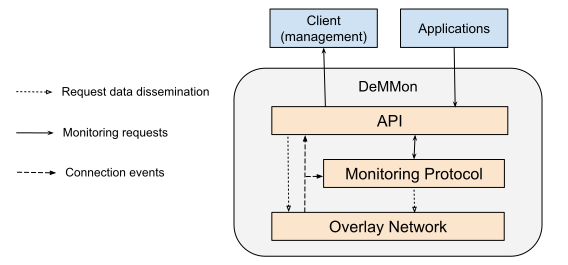
\includegraphics[width=\textwidth]{Chapters/Figures/DeMMon-arch-overview.pdf}
    \caption{An overview of the architecture of DeMMon}
    \label{fig:demmon-overview}
\end{figure}
    
First, the \textbf{API} exposes the functionality of the framework, its main objectives are to: (1) allow issuing commands to collect metrics about nodes (or services they host) in the system; (2) allow those metrics to be queried through the use of a query language; (3) allow registering alarms which trigger based on conditions which evaluate the collected information. It is important to notice that the API is not the component tasked with gathering the information to perform these tasks, instead, the API's purpose is to expose the results and mediate the interactions between the clients and the remaining modules.

Second, the \textbf{monitoring module} which is tasked with storing metrics, resolving queries regarding stored metrics, removing expired metrics, and periodically evaluating registered alarms and triggering callbacks which the API then propagates to the client. This module, toghether with the API, satisfies points (\ref{enum:demmon_4} and \ref{enum:demmon_6}) of the aforementioned requirements.

The \textbf{overlay network} strives to build a latency-aware multi-tree-shaped network. Nodes in this network use latency, node capacity, and a set of logical rules to change their location either from one tree to another or within their tree until they have an optimized set of nodes (according to latency). The connections resulting from the operation of this protocol are the basis for the aggregation protocol. In addition, this module also offers limited horizont flood techniques, exposed through the API, fulfilling the points \ref{enum:demmon_1} and \ref{enum:demmon_5} of the requirements.

Finally, the \textbf{aggregation protocol} is a component that performs on-demand metric collection based on issued commands from the API. This component takes advantage of the overlay networks' established connections and hierarchical structure to perform efficient distributed aggregations. It allows three types of decentralized aggregation: (1) tree aggregation, which consists of collecting metrics and merging them using the tree, collecting a globally aggregated value in the tree roots, or a partial view of the system for nodes which are not the root of the overlay); (2) global aggregation, where nodes also use their tree connections to efficiently collect an aggregated global value (independently of being the root of the tree); and (3) neighborhood aggregation, where nodes collect values (non aggregated) of nearby nodes in term of hop proximity. These three mechanisms satisfy points \ref{enum:demmon_2} and \ref{enum:demmon_3} of the aforementioned requirements. 

In the following sections we will provide a detailed explanation of each individual module, starting by the \textbf{overlay network} (section \ref{sec:overlay_network}), followed by \textbf{aggregation protocol} (section \ref{sec:mon_protocol}), and lastly, the \textbf{monitoring module} (section \ref{sec:mon_module}) and \textbf{API} (section \ref{sec:api}). 

\section{Overlay network} 
\label{sec:overlay_network}

\input{Chapters/membership/pseudocode/jlt-pseudocode.tex}

In this section, we discuss the design of the overlay network, which aims to build and maintain a latency and capacity-aware tree-shaped network (capacity represents one, or a combination of, values that denote the node's computing and networking power). We begin by providing the considered system model, then follow with an overview of the mechanisms responsible for building and maintaining the tree. Lastly, we conclude the chapter with a summary and discussion of the protocol.

\subsection{System Model}

The assumed system model is assumed to be a distributed scenario composed of nodes connected to the internet set-up such that they can send and receive messages via the internet (with an external IP or port-forwarding). We also assume that nodes are spread throughout a large area and have varied capacity values.

Regarding the fault model, we assume that all but a small portion of nodes (also known as the landmarks, which in our model represent DCs) can fail, and when other nodes fail, they do so in a crash-fault manner, stopping all emissions and receptions of messages. We assume landmarks have additional fault tolerance given their privileged infrastructure, and additionally, we assume other such as replication \cite{} mechanisms could be employed to ensure that faulty landmarks get replaced in case of failure. 
  
Finally, all nodes must run the same software stack with similar configuration settings and landmark values, installed a priori.

\subsection{Overview}

As previously mentioned, the main objective of the created protocol is to establish a latency and capacity-aware multi-tree-shaped network, rooted on the previously mentioned landmarks. Our motivations for choosing the tree structure for the network are the following: (1) to map the cloud-edge environment, by rooting the trees on nodes running DCs in the cloud, and creating a hierarchical structure for other, less powerful, nodes to be coordinated from the roots \todo{isto e esticar?} (2) to be able to map the heterogeneity of each device in the environment: by biasing the placement of nodes in the tree such that nodes with higher capacity are placed higher in the tree, and nodes with lower capacity are biased towards lower levels of the tree, nodes are used more or less according to their capacity values; (3) the tree structure can be easily employed to perform efficient aggregations, by propagating and merging values recursively from the lower to the higher levels of the tree, which is the basis for the aggregation protocol presented in \todo{add ref}; and finally, (4) by leveraging on the tree structure, nodes can propagate information efficiently, given that, in a network composed of N nodes, broadcasts require only N-1 message transmissions to reach all nodes in the network. 

The tree structure the protocol aims to establish and maintain can be observed in figure \todo{criar imagem para ilustrar estrutura resultante}, which, as previously referenced, is composed of multiple trees, and these are connected through their respective landmarks. The nodes connected to the landmarks, (denoted their \textbf{children}), may or may not form themselves be the parent of their own children. Intuitively, the \textbf{grandparent} of a certain node is their parents' parent, and the descendants of a certain node are constituted by all its children, and childrens' children, recursively. All nodes who share the same parent (\textbf{siblings}) are connected among themselves, forming a \textbf{group}, whose size is biased (but not guaranteed) to be within two configurable upper and lower bounds. Therefore, all nodes have active connections to their parent, children and siblings, this group of nodes denotes a node's \textbf{active view}. Nodes also have have knowledge of other nodes in the network, acquired via periodic semi-random periodic walks, which we will describe ahead. 

The devised algorithm is composed by three main mechanisms: (1) the \textbf{join} mechanism, which aims to establish the initial tree structures, (2) the \textbf{active view maintenance}, responsible for bounding the number of connections for each node, and optimizing the connections of each node, (3)  and finally \textbf{passive view maintenance}, responsible for collecting information about peers which are not in the active view, which are used for both fault tolerance and connection optimizations.

\subsubsection{Join mechanism}

The Join mechanism is the mechanism responsible for choosing the initial parent connection, which performs a greedy depth-first search to find a suitable low latency node in the network with more than zero children. This mechanism is the first to be executed by all nodes in the system, with the pseudocode presented in algorithm \ref{alg:memb:join}. 

% JOIN -----

\begin{algorithm}{}
\caption{Join Protocol} \label{alg:memb:join}
    % \setstretch{0.85}
\begin{algorithmic}[1]
    \asdtypes
        \State Node : <lat, parentIP, nrChildren, replied, IP, ID, coords, version, children<IP,  nrChildren\>\>
    \asdend
    \asdstate \label{alg:memb:join:state}
        \State contactedNodes \Comment{collection of all successfully contacted nodes}
        \State nodesToContact \Comment{nodes being contacted}
        \State landmarks \Comment{landmark nodes}
        \State joinTimeouts \Comment{collection of contacted nodes -> timerIDs}
        \State bestPeerLastLevel : Node \Comment{the best peer contacted so far in the join process}
        \State joinReqTimeoutTid \Comment{ timerID for join messages}
        \State self : Node \Comment{ myself}
    \asdend

\asdupon[Init(landmarks : IP[], selfIP, isLandmark)] \label{alg:memb:join:init}
    \State landmarks \asdassign landmarks 
    \State joinTimeouts, prevBestP \asdassign \{\}, nil
    \IfThenElse{isLandmark}
    {addLandmarkUntilSuccess(landmarks) \label{alg:memb:join:add_land}} 
    {contactNodes(landmarks) \label{alg:memb:join:contact_landm}} 
\asdend


\asdupon[receive(Join<>,sender)] \label{alg:memb:join:recv_join}
    \State sendMessageSideChannel(JoinReply<self.parent, self.node, self.children>, sender) 
\asdend
    
\asdupon[receive JoinReply(<parentIP, node, children>, sender) \&\& measuredLatency(lat)]  \label{alg:memb:join:recv_join_reply}
        \If{\asdin{node.IP}{nodesToContact}} 
            \If{\asdin{parentIP}{Landmarks}}
                \State self.coordinates[getIdx(landmarks, sender)] = lat
            \EndIf
            \State nodesToContact[node.IP].lat \asdassign lat
            \State nodesToContact[node.IP].children \asdassign children
            \State nodesToContact[node.IP].parent \asdassign parentIP
            \State nodesToContact[node.IP].replied \asdassign true
            \State cancelTimer(joinTimeouts[sender])
            \State delete(joinTimeouts, sender)
        \Else
            \State nodesToContact.delete(node)
        \EndIf
\asdend

\asdupon[(forall n $\in$ nodesToContact -> n.replied)] \label{alg:memb:join:cond_go}
    \State contactedNodes.appendAll(nodesToContact)
    \For{node in sortedByLatency(nodesToContact)}
        \If{(\asdnotin{node.IP}{landmarks}) \&\& node.nrChildren == 0} \label{alg:memb:join:verif_children}
            \State continue \Comment{check if node has enough children}
        \EndIf
        \If{prevBestP != nil \&\& (prevBestP.lat $\le$ node.lat || prevBestP.nrChildren < config.minGroupSize)} \label{alg:memb:join:verif_vs_prev}
            \State joinAsChild(prevBestP)
        \Else
            \State prevBestP \asdassign node \label{alg:memb:join:advance}
            \State toContact \asdassign [\asdin{c}{prevBestP.children} -> c.nrChildren > 0]
            \State contactNodes([c.IP for c in toContact])
        \EndIf
        \State return
    \EndFor
    \IfThenElse{prevBestP != nil} 
    {joinAsChild(prevBestP)}  
    {abortJoinAndRetryLater()} \label{alg:memb:join:join_base_case}
    \State return
\asdend

\asdupon[JoinTimeoutTimer(node) || NodeMeasuringFailed(node)] \label{alg:memb:join:exclusions}
    \IfThenElse{(L in Landmarks)}{abortJoinAndRetryLater()}{delete(nodesToContact[L])} 
\asdend

\asdupon[JoinRequestTimer(p : Node)]
    \If {sender == prevBestP}
        \If{p.parentIP != nil}
            \State prevBestP \asdassign contactedNodes[p.parentIP]
            \State joinAsChild(prevBestP)
        \Else
            \State abortJoinAndRetryLater()
        \EndIf
    \EndIf
\asdend

\asdupon[receive(JoinRequest<>, sender)]
    \State childID \asdassign addChildren(sender) \Comment{new chilren is established, and an ID is generated for it}
    \State sendMessageSideChannel(JoinRequestReply<childID, self>, p.IP)
\asdend
    
\asdupon[receive(JoinRequestReply<myID, parent>, sender)]
    \If {sender == prevBestP} 
        \State parent \asdassign sender \Comment{Adds Parent is established, join complete}
        \State cancelTimer(joinReqTimeoutTid)
        \State self.ID \asdassign parent.ID + "/" + myID \Comment{Later used in shuffle mechanism}
    \EndIf
\asdend

\asdprocedure[joinAsChild(p : Node)]
    \State joinReqTimeoutTid \asdassign setupTimer(JoinRequestTimer<p>, config.JoinTimeout)
    \State sendMessageSideChannel(JoinRequest<>, p.IP)
\asdend

\asdprocedure[contactNodes(ips : IP[])]
    \State nodesToContact \asdassign \{\}
    \State toContact \asdassign [Node<0,nil,0,false,lIP,false,[]> for ip in ips]
    \For{n in toContact}
        \State nodesToContact[n] \asdassign n
        \State MeasureNode(n) 
        \State sendMessageSideChannel(JoinMessage<>, n)
        \State joinTimeouts[n] \asdassign \asdassign setupTimer(JoinTimeoutTimer(n), config.JoinTimeout)
    \EndFor
\asdend

\end{algorithmic}
\end{algorithm}


Its first step (line \ref{alg:memb:join:state}) is to initialize the state of the joining node, composed by: (1) a map of type Node containing all successfully contacted nodes so far the join process, (2) a collection of type Node and a set of timer ids for each contacted node, (4) the best node contacted so far in the join process, (5) a timer id for contacting the chosen node in the join process, and finally (5) a variable of type Node denoting the peer itself. The type ``Node'' is a collection of attributes regarding a node, composed of latency measured, its current parent, number of children, whether the node replied to the message, its IP, and an array of its childrens' IP and children number.

Then, each node joins the system, the procedures taken to join the tree differ consonant the node is a landmark or not. Given that landmarks are the roots of the trees, they have no parent in the resulting overlay, and consequently, in the join algorithm, these nodes attempt to repeatedly establish a connection with other landmarks by sending a special message. Landmarks that receive this message will send a reply and establish a connection back (line \ref{alg:memb:join:add_land}), a joining landmark node only stops sending messages to other landmarks when the respective reply is received.

Nodes that are not landmarks begin the process of choosing their initial parent, initiated by sending a JOIN message via a temporary TCP channel, measuring the latency, and issuing ``joinTimers'' for all tree roots (line \ref{alg:memb:join:contact_landm}), then the node awaits the responses from the contacted nodes, during this process, the joining node listens for any ``joinTimers'' which have triggered, or until any of the node measurements has been unsuccessful (meaning contacted nodes have exceeded their reply timeout), if this happens, in the case of the contacted node being a landmark, the joining node aborts the join process and waits a configurable amount of time until attempting to re-join the overlay again. If the timed-out node is not a landmark, then that node is excluded from the remaining of the join process, and the join process is resumed as normal (line \ref{alg:memb:join:exclusions}).

When a node receives a JOIN message, it sends a JOINREPLY message back to the original sender containing: its parent, itself, and its children (line \ref{alg:memb:join:recv_join}). When the joining node receives the joinReply, it checks to see if it is not from a timed out node, or if the node's parent is not the same anymore, if any of these conditions are observed, then the reply is discarded. 

Then, whenever the joining node has either: received the JOINREPLY messages from all the contacted nodes, and stored the information (line \ref{alg:memb:join:recv_join_reply}), or they have been timed-out via the ``joinTimers'', it evaluates all contacted nodes, attempting to find the contacted node with the lowest latency which is a suitable parent by performing the following verifications:

\begin{enumerate}
    \item Verify if the node already has any children or if the node is a landmark (and can become parent of the joining node) (line \ref{alg:memb:join:verif_children}).
    
    \item Verify if there was a node already contacted which was a suitable parent and had lower latency, if there was, the joining node sends a JOINREQUEST and sets up a ``JoinRequestTimer'' for that node, and stops the verification process. (line \ref{alg:memb:join:verif_vs_prev})

    \item Verify if the current node has both enough children, and has the lowest latency up to this point in the join process, then the joining node assigns it as its best node so far and starts a new recursive step by sending JOIN messages and measuring the children of that node which themselves have more than one children (line \ref{alg:memb:join:advance}). Note that if none the current nodes' children are suitable parents (i.e. have no children themselves), then the condition in line \ref{alg:memb:join:cond_go} is triggered and the joining node will request the current best node to be its parent.
\end{enumerate}

If none of the verified peers was suitable to start a new recursive step (line \ref{alg:memb:join:join_base_case}) (either had no children or all verified nodes had higher latency than a previously contacted node), then the node joining node sends a ``JoinRequest'' to that node and sets up a ``JoinRequestTimer'' for the best previously contacted node (any node which receives a ``JoinRequest'' message replies with a ``JoinRequestReply''). 

The join process is concluded with both the reception of a ``JoinRequestReply'' and the establishment of the connection between the sender and receiver of the message. If the ``JoinRequestTimer'' timer triggers while waiting for the response, the node will recursively fall back to the parent of the selected node or re-join the overlay later in case there is no parent available. 

\subsubsection{Active view maintenance}

The second mechanism of the devised membership algorithm, called active view maintenance, is the mechanism responsible for maintaining the size of the groups. It achieves this by choosing new parents to form new groups using latency and node capacity as heuristics for the choice. This mechanism is coordinated by each parent, and is only done when the group exceeds its size limit. The information necessary to feed this mechanism is transmitted periodically from each children to their parents. 

The pseudocode for this mechanism is presentend in algorithm \ref{alg:memb:active_view_maint}, and starts by defining the necessary state: the nodes' active view (parent, children, and siblings), and an auxiliary map of sets, which holds the latencies of each children to every other children. (lines \ref{alg:memb:active_view_maint:state_start}-\ref{alg:memb:active_view_maint:state_end}). 

The mechanism starts with the propagation of information from the parent to the children and vice-versa. As observable in lines \ref{alg:memb:active_view_maint:update}-\ref{alg:memb:active_view_maint:update_end}), each parent transmits to its children a list of its current siblings, and propagates to its parent the latency to each of its siblings. Then, when this information is received (lines \ref{alg:memb:active_view_maint:update_recv_par} and \ref{alg:memb:active_view_maint:update_recv_chi}), it is merged into their local states for later use.

The second part of this mechanism is also periodic and is responsible for maintaining the group sizes by creating new groups, or sending children to already created groups (line \ref{alg:memb:active_view_maint:update_eval}) when necessary, this mechanism is only executed if the number of children exceeds the configured maximum number of children per parent (in order to keep group sizes close to full). Each node starts by merging all of its received latency pairs into a single set, where the node with the highest capacity is the first node of each pair (lines \ref{alg:memb:active_view_maint:update_eval_merge_start}-\ref{alg:memb:active_view_maint:update_eval_merge_finish}). Then, it iterates the added edges set by ascending order of latency, making the following steps:

\begin{enumerate}
    \item If the number of current children minus the nodes already sent to a lower level is lower than the middle point between the maximum size of a group, then the node concludes the mechanism (line \ref{alg:memb:active_view_maint:check_done_1})
    
    \item if the latency of the node pair that is being observed is higher than the parents latency to it, meaning it raises the overall latency of the system, and the current node size is lower than the configured maximum, then the process is concluded. (line \ref{alg:memb:active_view_maint:check_done_2})
    
    \item If any of the nodes was already sent to lower levels of the tree, then the current edge is skipped (line \ref{alg:memb:active_view_maint:check_done_3})
    
    \item Then, if the node wigh higher capacity of the edge pair has no children yet, the lower capacity node is added to its ``possibleChildren'' set, when this set has the same size of the minimum configured group size (i.e. the hifgher capacity node has enough candidates to form a new group), then the 
\end{enumerate}


\begin{algorithm}
    \caption{Membership protocol (Active view Optimization)} \label{alg:memb:active_view_maint}
    % \setstretch{0.85}
    \begin{algorithmic}[1]
        \asdstate
            \State parent \Comment{defined in join} \label{alg:memb:active_view_maint:state_start}
            \State children \Comment{defined in join} 
            \State siblings  
            \State childrenLatencies : dict<string:dict<string:number>> \label{alg:memb:active_view_maint:state_end} \Comment{Holds the latencies of each children to every other children}
        \asdend

        \asdrepeateveryx{config.updatePeriodicity} \label{alg:memb:active_view_maint:update}
            \If{parent != nil}
                \State sLatencies \asdassign set()
                \For{sibling in siblings}
                    \State sLatencies.append(<sibling.IP,sibling.measuredLatency)
                \EndFor
                \State sendMessage(UpdateChildStatus<children, siblingLatencies>, parent)
            \EndIf
            \For{child in chidren}
                \State sendMessage(UpdateParentStatus<self, chidren \\ child>)
            \EndFor
        \asdend \label{alg:memb:active_view_maint:update_end}

        \asdupon[receive(UpdateParentStatus<parent, children>, sender)] 
        \label{alg:memb:active_view_maint:update_recv_par}
            \If{sender == parent.IP}
                \State parent \asdassign parent
                \State self.ID \asdassign parent.ID + myID
                \State grandParent \asdassign grandParent
                \State siblings \asdassign siblings
            \EndIf
        \asdend

        \asdupon[receive(UpdateChildStatus<child, childSiblingLatencies>, sender)]\label{alg:memb:active_view_maint:update_recv_chi}
            \If{children[sender] != nil}
                \State children[sender]\asdassign child
                \State childrenLatencies[sender] \asdassign childSiblingLatencies
            \EndIf
        \asdend

        \asdrepeateveryx{config.evalGroupSize} \label{alg:memb:active_view_maint:update_eval}
            \If{len(children) <= config.maxGroupSize}
                \State return
            \EndIf
            \State childrenLatValues \asdassign set()
            \For{c1 in children} \label{alg:memb:active_view_maint:update_eval_merge_start}
                \For{<c2, lat> in childrenLatencies[c]}
                    \If{lat - c1.measuredLatency > d.config.maxLatDowngrade}
                        \State continue
                    \EndIf
                    \State isDowngrade \asdassign lat > c1.measuredLatency
                    \IfThenElse{c1.cap > c2.cap}
                    {childrenLatValues.add(<c1,c2,lat,isDowngrade>)}
                    {childrenLatValues.add(<c2,c1,lat,isDowngrade>)}
                \EndFor
            \EndFor \label{alg:memb:active_view_maint:update_eval_merge_finish}
            \State kickedNodes, newParents \asdassign set(),set()
            \State pChildren \asdassign dict<string,set<Node{>}{>} \Comment{set of potential children for each children}
            \State sortByLatency(childrenLatValues)
            \State idealGroupSize \asdassign config.maxSize - config.MinGroupSize
            \For{<c1,c2,lat,isDowngrade> in childrenLatValues}
                \If{len(children) - len(kickedNodes) <= idealGroupSize} \label{alg:memb:active_view_maint:check_done_1}
                    \State break
                \EndIf
                \If{len(children) - len(kickedNodes) <= config.maxSize \&\& isDowngrade} \label{alg:memb:active_view_maint:check_done_2}
                    \State break
                \EndIf
                \If{\asdin{c1}{kickedNodes} || \asdin{c2}{kickedNodes} ||  \asdin{lowerCapC}{newParents}} \label{alg:memb:active_view_maint:check_done_3}
                    \State continue
                \EndIf
                \If{c1.nrChildren == 0 \&\& newParents[c1] == nil}
                    \State pChildren[c1].append(c2)
                    \If{len(pChildren) >= config.MinGroupSize}
                        \If{len(children) - len(kickedNodes) - len(pChildren) > idealGroupSize || len(pChildren) >= config.maxSize}
                            \For{potentialChild in pChildren[c1]}
                                \State newParents <- newParents + c1
                                \State send(OptimizationPropose<c1>, potentialChild)
                                \State c1.nrChildren++
                                \State kickedNodes <- kickedNodes + potentialChild
                            \EndFor
                            \For{<nIP,pontentialChildrenTmp> in pChildren}
                                \State pontentialChildrenTmp.deleteAll(pChildren[c1])
                            \EndFor
                            \State pChildren[c1] \asdassign set<Node>
                            \State continue
                        \EndIf
                    \EndIf
                \Else
                    \State kickedNodes <- kickedNodes + c2
                    \State send(OptimizationPropose<higherCapNode>, lowerCapNode)
                \EndIf    
            \EndFor
        \asdend

        \asdupon[receive(OptimizationPropose<newParent>, sender)]
            \If{sender == parent}
                \State send(OptimizationProposeRequest<sender>, newParent)
            \EndIf
        \asdend

        \asdupon[receive(OptimizationProposeRequest<p>, sender)]
            \If{ p == parent \&\& sender in siblings} \Comment{ parent issuing the message is the same parent that i have}
                \State send(OptimizationProposeRequestReply<true>, sender)
            \Else
                \State sendSideChannel(OptimizationProposeRequestReply<false>, sender)
            \EndIf
        \asdend

        \asdupon[receive(OptimizationProposeRequestReply<reply>, sender)]
            \If{reply}
                \State sendMessageAndDisconnectFrom(DisconnectMessage<>, parent)
                \State addParent(sender)
            \EndIf
        \asdend

    \end{algorithmic}
\end{algorithm}


\subsubsection{Passive view maintenance}
\begin{algorithm}
\label{alg:memb:passive_view_maint}
\caption{Membership protocol (Passive view maintenance)}
\begin{algorithmic}[1]
    
    \asdstate
        \State pView : set<Node> \label{alg:memb:passive_view_maint:state}
    \asdend

    \asdrepeateveryx{config.RandWalkPeriodicity} \label{alg:memb:passive_view_maint:walk_trig}
        \State sample \asdassign getRandSample([pView + allNeighs + children + parent + siblings], config.NrPeersToMergeRandWalk)
        \State target \asdassign getRand(excludeDescendatsOf(ascNeighs, self.ID))
        \State sendMessage(RandomWalk<sample + self, config.RandWalkTTL, self.ID, self.IP>, target)
    \asdend

    \asdupon[receive( RandomWalk<sample, ttl, nID, orig>, sender)] \label{alg:memb:passive_view_maint:walk_rec}
        \State nrNodesToRemove \asdassign config.NrPeersToMergeRandWalk
        \If{config.RandWalkTTL - ttl < config.NrStepsToIgnore}:
            \State nrNodesToRemove \asdassign 0
        \EndIf
        \State updateNodesToHigherVersion(sample, pView) \label{alg:memb:passive_view_maint:walk_rec_merge_start}
        \State ascNeighs \asdassign set(parent + siblings)
        \State allNeighs \asdassign set(allNeighs + ascNeighs + children)
        \State toAdd \asdassign getRandSample(excludeDescendantsOf(pView + allNeighs / sample,self.ID), config.NrPeersToMergeRandWalk)
        \State toRemoveFromSample \asdassign getRandSample(sample, nrNodesToRemove)
        \State sample \asdassign sample / toRemoveFromSample
        \State pView \asdassign excludeDescendantsOf(toRemoveFromSample + pView, self.ID)  
        \State pView \asdassign pView / allNeighs
        \State pView \asdassign pView[:config.MaxEViewSize]
        \State sample  \asdassign trimSetToSize(sample + toAdd + self, config.MaxRndWalkSampleSize) \label{alg:memb:passive_view_maint:walk_rec_merge_end}
        \State target \asdassign getRand(excludeDescendantsOf(allNeighs, nID)
        \If{target == nil || ttl == 0} \label{alg:memb:passive_view_maint:walk_rec_send}
            \State sendMessageSideChannel(RandomWalkReply<sample>, orig)
        \Else
            \State sendMessage(RandomWalk<sample, ttl-1, nID, orig>, getRandom(ascNeighs))
        \EndIf \label{alg:memb:passive_view_maint:walk_rec_send_end}
    \asdend

    \asdupon[receive( RandomWalkReply<sample>, sender)]: \label{alg:memb:passive_view_maint:walk_reply_recv_start}
        \State sample \asdassign excludeDescendantsOf(sample, self.ID)
        \State updateNodesToHigherVersion(sample, pView)
        \State sample \asdassign excludeNodesInActiveView(sample)
        \State pView \asdassign trimSetToSize(pView + sample, config.MaxEViewSize) \label{alg:memb:passive_view_maint:walk_reply_recv_end}
    \asdend


    \asdrepeateveryx{config.OportunisticOptimizationTimeout} \label{alg:memb:passive_view_maint:eval_nodes}
        \State toMeasureRand \asdassign getRandSample(pView, len(pView)) // shuffle sample
        \State toMeasureBiased \asdassign sortByEuclideanDist(pView / toMeasureRand)

        \State measuredNr \asdassign 0
        \For{i=0; i < len(toMeasureRand) \&\& measuredNr < config.ToMeasureRand ; i++}
            \If{canBecomeChildrenOf(p)} \label{alg:memb:passive_view_maint:opt_verification_1}
                \State measuredNr++
                \State measurePeer(p)
            \EndIf
        \EndFor
        \State measuredNr \asdassign 0
        \For{i=0; i < len(toMeasureRand) \&\& measuredNr < config.toMeasureBiased ; i++}
            \If{canBecomeChildrenOf(p)} \label{alg:memb:passive_view_maint:opt_verification_2}
                \State measuredNr++
                \State measurePeer(p)
            \EndIf
        \EndFor
    \asdend

    \asdupon[peerMeasured(p, latency)] \label{alg:memb:passive_view_maint:peer_measured}
        \State latencyImprovement := parent.measuredLatency - Latency
        \If{latencyImprovement >= config.MinLatencyForImprovement}
            \State sendMessageSideChannel(OportunisticImprovementReq<self>,p)
        \EndIf
    \asdend

    \asdupon[receive(OportunisticImprovementReq<p>,sender)] \label{alg:memb:passive_view_maint:oport_msg_recv}
        \If{isDescendent(p.ID,self)}
            \State sendMessageSideChannel(OportunisticImprovementReqReply<false>,sender)
        \Else
            \State addChildren(sender)
            \State sendMessageSideChannel(OportunisticImprovementReqReply<true>,sender)
        \EndIf
    \asdend

    \asdupon[receive(OportunisticImprovementReqReply<answer>,sender)] \label{alg:memb:passive_view_maint:op_msg_reply_recv}
        \If {answer} 
            \State disconnectFromCurrentParent(parent)
            \State addParent(sender)
        \EndIf
    \asdend

    \asdprocedure[canBecomeChildrenOf(c, parent)]
        \If{(c.nrChildren > 0 \&\& parent.ID.level() >= c.ID.level())}
            \State return false
        \EndIf
        \State return parent.nrChildren > 0 \&\& !isDescendentOf(parent.ID, c) \&\& !isDescendentOf(c, parent.ID)
    \asdend

    \asdprocedure[isDescendentOf(nodeID, PotentialDescID)]
        \State return PotentialDescID.Contains(nodeID)
    \asdend

\end{algorithmic}
\end{algorithm}

\subsection{Summary}

\section{Monitoring protocol}

\subsection{Overview}

\subsection{Aggregation mechanisms}

\subsubsection{Single root aggregation}

\subsubsection{Multi root aggregation}

\subsubsection{Neighborhood aggregation}

\subsection{Summary}

\section{API}

\subsection{System Model}

\subsection{Overview}

\subsection{Showcase}

\section{Aggregation protocol}
\label{sec:mon_protocol}

With a membership protocol capable of coordinating nodes into building a tree overlay network, a new range of options open for both the dissemination and aggregation of information. In this section, we discuss the devised decentralized aggregation protocol, which leverages on the tree structure to enable the on-demand collection of information (or metrics) in a decentralized manner. While in this work we present the protocol leveraging the overlay protocol defined in \ref{sec:overlay_network}, it is important to notice that the protocol is agnostic to which overlay protocol is executing, as long as it has the following characteristics: (1) it forms one or more network-shaped trees whose roots are interconnected, nodes in this tree must be connected to their parents, children and siblings (active view) in a bidirectional manner, and must provide callbacks for each node that is added or removed from the nodes's active view.

This protocol provides three different types of decentralized aggregation techniques, inspired from the study of the state of the art: (1) tree aggregation, (2) neighbourhood aggregation, and finally, (3) global aggregation, which we now clarify in further detail, starting by tree aggregation.

\subsection{Tree aggregation} \label{sec:mon_protocol:tree_agg}

Tree aggregation is the mechanism responsible for collecting metrics and merging them using the tree, collecting an aggregated value for all nodes which are descendants of the node performing this mechanism (also denoted the \textbf{root of the aggregation tree}). It is important to notice that this mechanism is executable by all nodes in the mechanism, and if two different nodes are aggregating the same values with the same parameters, and a node is descendent of the other, the descendant node, will, when possible, embed its tree into the ascendants' (thus not performing the mechanism individually for nodes with overlapping trees, and reusing the values of the already existing tree).

The pseudocode for this mechanism (as defined in \ref{alg:mon:tree_agg}) begins by defining the necessary state (line \ref{alg:mon:tree_agg:state}) for its execution, starting by the active view, composed of the parent, children, and siblings of the node, this state is maintained by the overlay protocol and changes to it are propagated through notifications (this process is omitted from the pseudocode). Then, it declares three maps, the first contains the necessary metadata for each aggregation tree, values of this map contain: (1) the height of the tree, (2) the merge function, (3) the query to generate local values, (4) the periodicity to export values (5) a boolean value representing if the value should be exported locally, (6) a boolean representing if the parent is also in the tree (and the node must propagate values to it or not), and finally (7) the ID of the tree from the parent's perspective (or nil, if the parent is not in the tree).

\begin{algorithm}
\caption{Tree aggregation} \label{alg:mon:tree_agg}
\begin{algorithmic}[1]

    \asdstate \label{alg:mon:tree_agg:state}
        \State parent,children,siblings \Comment{Defined by the overlay protocol}
        \State tIds \asdassign map()
        \State lastSeen \asdassign map()
        \State childValues \asdassign map()
    \asdend

    \asdupon[StartTreeAggregationRequest(tHeight, mergeF, query, periodicity ,outmName)] 
    \label{alg:mon:tree_agg:start_req}
        \State tId \asdassign hash(tHeight + mergeF + query + periodicity + outmName) \label{alg:mon:tree_agg:start_req_start}
        \If{tId in tIds} 
            \State <tHeight, mergeF, query, periodicity, outmName, timerId, isLocal, isParentSub, ptId> \asdassign tIds[tId]
            \State tIds[tId] \asdassign <tHeight, mergeF, query, periodicity, outmName, timerId, true, isParentSub, ptId>
        \Else:
        \State timerId \asdassign registerPeriodicTimer(ExportTreeAggTimer(tId), periodicity)
        \State tIds[tId] \asdassign <tHeight, mergeF, query, periodicity, outmName, timerId, true, false, nil>
        \EndIf\label{alg:mon:tree_agg:start_req_end}
    \asdend

    \asdupon[ExportTreeAggTimer(tId)] \label{alg:mon:tree_agg:export_trigger}
        \State <tHeight, mergeF, query, periodicity, outmName, timerId, isLocal, isParentSub, ptId> \asdassign tIds[tId]
        \If{isParentSub \&\& timeSince(tIdLastSeen[tId]) > config.treeAggExpiration}
            \If{!isLocal }
                \State tIds.delete(tId)
                \State lastSeen.delete(tId)
                \State cancelTimer(timerId)
                \State return
            \Else
                \State tIds[tId] \asdassign <tHeight, mergeF, query, periodicity, outmName, timerId, isLocal, false, nil>
            \EndIf
        \EndIf
        \State removeOldChildrenValues(childValues[tId])
        \State res \asdassign aggregateValues(mergeF, resolveQuery(query), childValues[tId])
        \If{isLocal}
            \State storeLocalVal(res, outmName)
        \EndIf 
        \If{isParentSub}
            \State sendMessage(PropagateTAggValues<ptId, res>, parent)
        \EndIf
    \asdend

    \asdupon[receive(PropagateTAggValues<tId, res>, sender)] \label{alg:mon:tree_agg:recv_propag_vals}
        \If{tId in tIds and sender in children}
            \If{tId not in childValues}
                \State childValues[tId] = map()
            \EndIf
            \State childValues[tId][sender] = res, time.Now()
        \EndIf
    \asdend

    \asdrepeateveryx{config.PropagateTAggTimeout seconds} \label{alg:mon:tree_agg:propag}
        \State toSendArr \asdassign set 
        \For{tId in tIds}
            \State <tHeight, mergeF, query, periodicity, outmName, timerId, isLocal, isParentSub, ptId> \asdassign tIds[tId]
            \If{isLocal}
                \State toSendArr.append(<max(tHeight -1, -1), mergeF, query, periodicity ,outmName, tId>)
            \EndIf
        \EndFor
        \For{c in chilren}        
            \State sendMessage(RefreshTreeAggFunc<toSendArr>, c)
        \EndFor
    \asdend

    \asdupon[receive(RefreshTreeAggFunc<tAggs>, sender)] \label{alg:mon:tree_agg:propag_recv}
        \If{parent == sender}
            \State toSendArr \asdassign set
            \For{<tHeight, mergeF, query, periodicity, outmName, ptId> in tAggs}
                \State tId \asdassign hash(tHeight + mergeF + query + periodicity + outmName)
                \If{id in tIds}
                    \State <tHeight, mergeF, query, periodicity, outmName, timerId, isLocal, isParentSub, ptId> \asdassign tIds[tId]
                    \State lastSeen[id] \asdassign time.Now()
                    \State tIds[tId] \asdassign <tHeight, mergeF, query, periodicity, outmName, timerId, isLocal, true, ptId>
                    \If{!isLocal \&\& <max(tHeight -1, -1) == -1 || <max(tHeight -1, -1) > 0}
                        \State toSendArr.append(<max(tHeight -1, -1), mergeF, query, periodicity ,outmName, timerId, tId>)
                    \EndIf
                \Else
                    \State toSendArr.append(<max(tHeight -1, -1), mergeF, query, periodicity ,outmName, timerId, tId>)
                    \State tIds[tId] \asdassign <tHeight, mergeF, query, periodicity, outmName, timerId, false, true, ptId>
                    \State registerPeriodicTimer(HandleTreeAggTimer(tId), periodicity)
                \EndIf
            \EndFor
            \For{c in chilren}        
                \State sendMessage(RefreshTreeAggFunc<toSendArr>, c)
            \EndFor
        \EndIf
    \asdend

    \end{algorithmic}
\end{algorithm}
    

Tree aggregation is started by the API sending a request to the protocol signalling the node should begin the procedure (line \ref{alg:mon:tree_agg:start_req}), this request contains: the maximum height of the tree, the merge function, the query to obtain the local value, the periodicity to execute the mechanism, and lastly, the resulting metric name. When a node receives this request, it generates a tree ID by hashing the concatenation of the tree height, the merge function, the query, the mechanism periodicity and finally the resulting metric name. This hashing is done so aggregation trees with different roots are embedded into each another, for example, if a certain node wishes to create an aggregation tree with height 5 rooted on itself, then, if a children of his (1 level lower) also creates an aggregation tree with height 4, the two trees will be embedded (as their ids will match), meaning the parent's aggregation results will be used to feed the locally requested values. It is important to notice that if the tree height is -1, then it is treated as if it had infinite height.

Before adding the tree to its local tree map, the node checks if there already is a tree with the same ID (meaning it has the same tree height, merge function, query, periodicity and resulting metric name) in the ``tIds'' map, if there is, then it sets the flag signalling the value should be exported locally, otherwise it adds a new entry to the map and sets up a periodic timer for that aggregation tree (lines \ref{alg:mon:tree_agg:start_req_start} to \ref{alg:mon:tree_agg:start_req_end}).

Whenever this timer triggers, (line \ref{alg:mon:tree_agg:export_trigger}), the node checks if the aggregation tree has expired (i.e. if the parent stopped refreshing the aggregation tree), if it it has, then the node cancels the timer and deletes the tree metadata, if it has not expired, then the node evaluates the query (this procedure will be explained in section \ref{sec:mon_module}), obtaining its local value, then it merges all the values sent by its children with its own using the merge function, producing the final aggregated result. Afterwards, if configured to do so, it will store the value locally, and if the parent is also subscribed to the aggregation tree, it propagates the obtained value to it. Whenever a node receives this propagation of values from another node (line \ref{alg:mon:tree_agg:recv_propag_vals}), it checks that it has the corresponding aggregation tree in its local set of trees and that the message was sent by its children, discarding it if it is not, and stores the received values into a map of maps, containing all children values for each aggregation tree.

Finally, each node periodically (using configured intervals) broadcasts to its children a message containing the aggregation trees it is the root of and that have height higher than 0 (line \ref{alg:mon:tree_agg:propag}). Whenever this message is received (line \ref{alg:mon:tree_agg:propag_recv}), the child merges all the received aggregation trees with registered ones, marking the parent as a subscriber for each previously present tree, and propagates the aggregation trees from which he is not the root of to its children.

\todo{talvez meter uma conclusão aqui?}

\subsection{Neighborhood aggregation}

Neighborhood aggregation is the mechanism responsible for collecting metrics from neighboring nodes to the node performing this mechanism, in essence, every node executing this mechanism creates a tree rooted upon itself by broadcasting messages with a configurable hop-based range periodically. Then, nodes who receive that message (essentially becoming federated in the tree) rebroadcast it to other peers and start to periodically propagate these values towards the root of each tree using the reverse path established by the broadcast message. Nodes in overlapping trees (i.e. propagating values derived from the same query) deduplicate the mechanisms of the propagation of broadcast messages and metric emission (by employing hashing, similarly to \ref{sec:mon_protocol:tree_agg}) in order to reduce the number of propagated messages.



\subsection{Global aggregation}

\subsection{Summary}


\section{Monitoring module}
\label{sec:mon_module}

The API is the last module of the devised framework. As previously mentioned, the purpose of this module is to expose the functionality of the remaining components of the framework by mediating the interactions between the clients and the remaining modules via well-defined operations. In this section, we provide a brief overview of the API implementation and detail its most relevant operations. 

\subsection{Overview}

This API is coalesced by a message-based protocol performed via WebSockets \todo{citation?}. The choice of using a message-based protocol is motivated by the fact that, contrary to traditional HTTP APIs, messages enable clients to receive events sent by the DeMMon servers. This feature is essential for both alerting (as triggered alarms need to be propagated to their issuing clients) and for issuing events such as active view changes to subscribed clients. Consequently, in this API, the client must first establish a connection with the server in order to perform operations, this is done via an HTTP server, which contains a single endpoint, used for establishing the WebSockets connection. In order to test the provided API and the capabilities of the framework, we also devised a client which performs the operations, available on \todo{put repo in}.

When connected, clients and servers exchange JSON formatted messages which may contain messages related to the behaviour of two types of operations: the first is a \textbf{request}, which is similar to an HTTP request, where the client creates a request and assigns it an ID which it sends to the deMMon server via a WebSockets message. When the server receives the message, it processes it and sends back to the client a reply message containing the ID and the reply contents using the same established connection. Requests are used, for example, for querying metrics. The second type of operation is a \textbf{subscription}, which initially performs similarly to a request, hovever, in this operation the server, posterior to the initial request, may send sporadic messages to the client containing events related to the issued subscription. This type of operation is used, for example, for both clients wanting to receive active view changes or for clients installing alarms and then receiving updates to changes in these alarms.

With this, we now provide a brief overview of what we believe to be the more relevant operations exposed by the deMMon API.

\subsubsection{API operations}

\begin{enumerate}
    \item \textbf{Install or remove buckets} These operations, as their name indicates, insert or remove buckets from the time series database. As previously mentioned in section \todo{ref}, buckets are containers for all time-series data with a certain name, periodicity and capacity. Whenever a ``create bucket'' operation is issued for a bucket with a name that collides with a pre-existing bucket (with a different periodicity), an error message is returned to the client.
    
    \item \textbf{Retrieve and insert metric values}. These two operations, performed via requests, add or extract values from the time series database. The insertion of values is performed using messages the metric values. When these messages are received, the values are inserted directly in the corresponding time series. The retrieval of metric values is also performed via a request containing a query in the devised query language. This query is passed to the monitoring module (specifically the metric engine) for processing. When the query has finished being processed by the metric engine, the result is sent back to the client via a message.
    
    \item \textbf{Subscription to active view updates}. This operation, as the name denotes, is performed via a subscription, where the initial reply contains the current view of the server. Then, whenever there is a change in the view of the deMMon server, it sends a message containing the change type (if either a new connection was established to a node, or if a previous connection disappeared).
    
    \item \textbf{Install continuous query}. This operation allows the installation of a continuous query. Continous queries are operations which contain multiple parameters, and are essentially queries that are evaluated at specified periodicities, and whose returning values are inserted into the time series database under a specified name. This operation is useful for applications that wish to, for example, resample their data to longer periodicities, or wish to calculate a certain aggregated value at specific intervals. 

    \item \textbf{Broadcast messages and subscribe to broadcast message receptions}. As the name indicates, these two operations refer to issuing and receiving broadcast messages. The emission of new broadcast messages is done via a request containing the message contents, the message TTL and the message ID (a text-based field). Whenever this request is received, the API sends a request to the overlay protocol, which in turn propagates the message contents via their active connections (until the TTL is 0). Broadcast messages are propagated and forwarded to peers in the active in a similar manner to the subscription messages (described in \todo{quote broadcast aggregation}). Finally, nodes can perform \textbf{Subscriptions to broadcast message receptions}, which are subscription operations for clients that wish to receive all messages with a certain ID that pass through the server's overlay protocol. 
    
    \item \textbf{Install Alarm}. This operation is coalesced by a subscription containing the parameters described in section \todo{citar seccao alarms}, whenever a client issues this operation, the API assigns a new ID to the alarm and adds it to the alarm manager (described in section \todo{ref}), where it begins being periodically verified. After this, if in any verification the alarm fires, the alarm manager notifies the API which in turn sends a message to the client with the firing alarm's ID.

    \item \textbf{Install and removal of neighborhood aggregation set}. These operations manage the operation of the neighborhood aggregation algorithm defined in section \todo{put ref to neigh agg}. These are performed via requests, in case of installation, these contain contain the parameters for the request mentioned in \todo{another ref to place}. Whenever the api receives a request for the creation of a neighborhood aggregation, it assigns an ID to it, and sends a reply to the client with the generated ID. Conversely, when the client no longer wishes to collect these values, it issues a removal request containing originally assigned ID of the aggregation set.

    \item \textbf{Install and removal of global aggregation function}. These operation initiate and stop the global aggregation procedure (described in subsection \todo{ref section global agg}), the behavior of this operation, in regard to the interaction betweeen the client and the server, is similar to the neighborhood aggregation set. However, nodes receiving this request become roots of their own global aggregation trees.

    \item \textbf{Install and remove tree aggregation function}. This is the last detailed operation of the deMMOn API, which in terms of interaction between the client and the server, behaves similarly to both the neighborhood and global aggregation requests. Whenever the API receives a request to begin global aggregation, it forwards it to the aggregation protocol, which begins the mechanism described in \todo{insert ref}.
\end{enumerate}

\todo{falar do cliente e do exporter}

\subsubsection{Summary}

In this section, we have presented an overview of the capabilities of the DeMMon API. We began by providing a brief overview of the interaction paradigm (message-based) and the reasons behind this choice. Next, we detailed the technologies used to realize this interaction paradigm and enumerated what we believe to be its most relevant operations. For each enumerated operation, we provided a brief explanation of its behaviour regarding both the effect on the remaining components and the model of interaction between the client and the server. 

\section{API}
\label{sec:api}

The API is the last module of the devised framework. As previously mentioned, the purpose of this module is to expose the functionality of the remaining components of the framework by mediating the interactions between the clients and the remaining modules via well-defined operations. In this section, we provide a brief overview of the API implementation and detail its most relevant operations. 

\subsection{Overview}

This API is coalesced by a message-based protocol performed via WebSockets \todo{citation?}. The choice of using a message-based protocol is motivated by the fact that, contrary to traditional HTTP APIs, messages enable clients to receive events sent by the DeMMon servers. This feature is essential for both alerting (as triggered alarms need to be propagated to their issuing clients) and for issuing events such as active view changes to subscribed clients. Consequently, in this API, the client must first establish a connection with the server in order to perform operations, this is done via an HTTP server, which contains a single endpoint, used for establishing the WebSockets connection. In order to test the provided API and the capabilities of the framework, we also devised a client which performs the operations, available on \todo{put repo in}.

When connected, clients and servers exchange JSON formatted messages which may contain messages related to the behaviour of two types of operations: the first is a \textbf{request}, which is similar to an HTTP request, where the client creates a request and assigns it an ID which it sends to the deMMon server via a WebSockets message. When the server receives the message, it processes it and sends back to the client a reply message containing the ID and the reply contents using the same established connection. Requests are used, for example, for querying metrics. The second type of operation is a \textbf{subscription}, which initially performs similarly to a request, hovever, in this operation the server, posterior to the initial request, may send sporadic messages to the client containing events related to the issued subscription. This type of operation is used, for example, for both clients wanting to receive active view changes or for clients installing alarms and then receiving updates to changes in these alarms.

With this, we now provide a brief overview of what we believe to be the more relevant operations exposed by the deMMon API.

\subsubsection{API operations}

\begin{enumerate}
    \item \textbf{Install or remove buckets} These operations, as their name indicates, insert or remove buckets from the time series database. As previously mentioned in section \todo{ref}, buckets are containers for all time-series data with a certain name, periodicity and capacity. Whenever a ``create bucket'' operation is issued for a bucket with a name that collides with a pre-existing bucket (with a different periodicity), an error message is returned to the client.
    
    \item \textbf{Retrieve and insert metric values}. These two operations, performed via requests, add or extract values from the time series database. The insertion of values is performed using messages the metric values. When these messages are received, the values are inserted directly in the corresponding time series. The retrieval of metric values is also performed via a request containing a query in the devised query language. This query is passed to the monitoring module (specifically the metric engine) for processing. When the query has finished being processed by the metric engine, the result is sent back to the client via a message.
    
    \item \textbf{Subscription to active view updates}. This operation, as the name denotes, is performed via a subscription, where the initial reply contains the current view of the server. Then, whenever there is a change in the view of the deMMon server, it sends a message containing the change type (if either a new connection was established to a node, or if a previous connection disappeared).
    
    \item \textbf{Install continuous query}. This operation allows the installation of a continuous query. Continous queries are operations which contain multiple parameters, and are essentially queries that are evaluated at specified periodicities, and whose returning values are inserted into the time series database under a specified name. This operation is useful for applications that wish to, for example, resample their data to longer periodicities, or wish to calculate a certain aggregated value at specific intervals. 

    \item \textbf{Broadcast messages and subscribe to broadcast message receptions}. As the name indicates, these two operations refer to issuing and receiving broadcast messages. The emission of new broadcast messages is done via a request containing the message contents, the message TTL and the message ID (a text-based field). Whenever this request is received, the API sends a request to the overlay protocol, which in turn propagates the message contents via their active connections (until the TTL is 0). Broadcast messages are propagated and forwarded to peers in the active in a similar manner to the subscription messages (described in \todo{quote broadcast aggregation}). Finally, nodes can perform \textbf{Subscriptions to broadcast message receptions}, which are subscription operations for clients that wish to receive all messages with a certain ID that pass through the server's overlay protocol. 
    
    \item \textbf{Install Alarm}. This operation is coalesced by a subscription containing the parameters described in section \todo{citar seccao alarms}, whenever a client issues this operation, the API assigns a new ID to the alarm and adds it to the alarm manager (described in section \todo{ref}), where it begins being periodically verified. After this, if in any verification the alarm fires, the alarm manager notifies the API which in turn sends a message to the client with the firing alarm's ID.

    \item \textbf{Install and removal of neighborhood aggregation set}. These operations manage the operation of the neighborhood aggregation algorithm defined in section \todo{put ref to neigh agg}. These are performed via requests, in case of installation, these contain contain the parameters for the request mentioned in \todo{another ref to place}. Whenever the api receives a request for the creation of a neighborhood aggregation, it assigns an ID to it, and sends a reply to the client with the generated ID. Conversely, when the client no longer wishes to collect these values, it issues a removal request containing originally assigned ID of the aggregation set.

    \item \textbf{Install and removal of global aggregation function}. These operation initiate and stop the global aggregation procedure (described in subsection \todo{ref section global agg}), the behavior of this operation, in regard to the interaction betweeen the client and the server, is similar to the neighborhood aggregation set. However, nodes receiving this request become roots of their own global aggregation trees.

    \item \textbf{Install and remove tree aggregation function}. This is the last detailed operation of the deMMOn API, which in terms of interaction between the client and the server, behaves similarly to both the neighborhood and global aggregation requests. Whenever the API receives a request to begin global aggregation, it forwards it to the aggregation protocol, which begins the mechanism described in \todo{insert ref}.
\end{enumerate}

\todo{falar do cliente e do exporter}

\subsubsection{Summary}

In this section, we have presented an overview of the capabilities of the DeMMon API. We began by providing a brief overview of the interaction paradigm (message-based) and the reasons behind this choice. Next, we detailed the technologies used to realize this interaction paradigm and enumerated what we believe to be its most relevant operations. For each enumerated operation, we provided a brief explanation of its behaviour regarding both the effect on the remaining components and the model of interaction between the client and the server. 

\section{Showcase}


% .
% It is important to notice that, as the nodes are organized in a tree, resource management systems may also take advantage of this structure to perform actions more efficiently, for example, using 

% such that nodes in higher levels of the tree have a broader knowledge of the whole system, and nodes in lower levels have more localized information. This feature is especially useful for frameworks that take advantage of the hierarchical structure to organize its nodes.

